% Options for packages loaded elsewhere
\PassOptionsToPackage{unicode}{hyperref}
\PassOptionsToPackage{hyphens}{url}
%
\documentclass[
]{book}
\usepackage{amsmath,amssymb}
\usepackage{lmodern}
\usepackage{iftex}
\ifPDFTeX
  \usepackage[T1]{fontenc}
  \usepackage[utf8]{inputenc}
  \usepackage{textcomp} % provide euro and other symbols
\else % if luatex or xetex
  \usepackage{unicode-math}
  \defaultfontfeatures{Scale=MatchLowercase}
  \defaultfontfeatures[\rmfamily]{Ligatures=TeX,Scale=1}
\fi
% Use upquote if available, for straight quotes in verbatim environments
\IfFileExists{upquote.sty}{\usepackage{upquote}}{}
\IfFileExists{microtype.sty}{% use microtype if available
  \usepackage[]{microtype}
  \UseMicrotypeSet[protrusion]{basicmath} % disable protrusion for tt fonts
}{}
\makeatletter
\@ifundefined{KOMAClassName}{% if non-KOMA class
  \IfFileExists{parskip.sty}{%
    \usepackage{parskip}
  }{% else
    \setlength{\parindent}{0pt}
    \setlength{\parskip}{6pt plus 2pt minus 1pt}}
}{% if KOMA class
  \KOMAoptions{parskip=half}}
\makeatother
\usepackage{xcolor}
\usepackage{color}
\usepackage{fancyvrb}
\newcommand{\VerbBar}{|}
\newcommand{\VERB}{\Verb[commandchars=\\\{\}]}
\DefineVerbatimEnvironment{Highlighting}{Verbatim}{commandchars=\\\{\}}
% Add ',fontsize=\small' for more characters per line
\usepackage{framed}
\definecolor{shadecolor}{RGB}{248,248,248}
\newenvironment{Shaded}{\begin{snugshade}}{\end{snugshade}}
\newcommand{\AlertTok}[1]{\textcolor[rgb]{0.94,0.16,0.16}{#1}}
\newcommand{\AnnotationTok}[1]{\textcolor[rgb]{0.56,0.35,0.01}{\textbf{\textit{#1}}}}
\newcommand{\AttributeTok}[1]{\textcolor[rgb]{0.77,0.63,0.00}{#1}}
\newcommand{\BaseNTok}[1]{\textcolor[rgb]{0.00,0.00,0.81}{#1}}
\newcommand{\BuiltInTok}[1]{#1}
\newcommand{\CharTok}[1]{\textcolor[rgb]{0.31,0.60,0.02}{#1}}
\newcommand{\CommentTok}[1]{\textcolor[rgb]{0.56,0.35,0.01}{\textit{#1}}}
\newcommand{\CommentVarTok}[1]{\textcolor[rgb]{0.56,0.35,0.01}{\textbf{\textit{#1}}}}
\newcommand{\ConstantTok}[1]{\textcolor[rgb]{0.00,0.00,0.00}{#1}}
\newcommand{\ControlFlowTok}[1]{\textcolor[rgb]{0.13,0.29,0.53}{\textbf{#1}}}
\newcommand{\DataTypeTok}[1]{\textcolor[rgb]{0.13,0.29,0.53}{#1}}
\newcommand{\DecValTok}[1]{\textcolor[rgb]{0.00,0.00,0.81}{#1}}
\newcommand{\DocumentationTok}[1]{\textcolor[rgb]{0.56,0.35,0.01}{\textbf{\textit{#1}}}}
\newcommand{\ErrorTok}[1]{\textcolor[rgb]{0.64,0.00,0.00}{\textbf{#1}}}
\newcommand{\ExtensionTok}[1]{#1}
\newcommand{\FloatTok}[1]{\textcolor[rgb]{0.00,0.00,0.81}{#1}}
\newcommand{\FunctionTok}[1]{\textcolor[rgb]{0.00,0.00,0.00}{#1}}
\newcommand{\ImportTok}[1]{#1}
\newcommand{\InformationTok}[1]{\textcolor[rgb]{0.56,0.35,0.01}{\textbf{\textit{#1}}}}
\newcommand{\KeywordTok}[1]{\textcolor[rgb]{0.13,0.29,0.53}{\textbf{#1}}}
\newcommand{\NormalTok}[1]{#1}
\newcommand{\OperatorTok}[1]{\textcolor[rgb]{0.81,0.36,0.00}{\textbf{#1}}}
\newcommand{\OtherTok}[1]{\textcolor[rgb]{0.56,0.35,0.01}{#1}}
\newcommand{\PreprocessorTok}[1]{\textcolor[rgb]{0.56,0.35,0.01}{\textit{#1}}}
\newcommand{\RegionMarkerTok}[1]{#1}
\newcommand{\SpecialCharTok}[1]{\textcolor[rgb]{0.00,0.00,0.00}{#1}}
\newcommand{\SpecialStringTok}[1]{\textcolor[rgb]{0.31,0.60,0.02}{#1}}
\newcommand{\StringTok}[1]{\textcolor[rgb]{0.31,0.60,0.02}{#1}}
\newcommand{\VariableTok}[1]{\textcolor[rgb]{0.00,0.00,0.00}{#1}}
\newcommand{\VerbatimStringTok}[1]{\textcolor[rgb]{0.31,0.60,0.02}{#1}}
\newcommand{\WarningTok}[1]{\textcolor[rgb]{0.56,0.35,0.01}{\textbf{\textit{#1}}}}
\usepackage{longtable,booktabs,array}
\usepackage{calc} % for calculating minipage widths
% Correct order of tables after \paragraph or \subparagraph
\usepackage{etoolbox}
\makeatletter
\patchcmd\longtable{\par}{\if@noskipsec\mbox{}\fi\par}{}{}
\makeatother
% Allow footnotes in longtable head/foot
\IfFileExists{footnotehyper.sty}{\usepackage{footnotehyper}}{\usepackage{footnote}}
\makesavenoteenv{longtable}
\usepackage{graphicx}
\makeatletter
\def\maxwidth{\ifdim\Gin@nat@width>\linewidth\linewidth\else\Gin@nat@width\fi}
\def\maxheight{\ifdim\Gin@nat@height>\textheight\textheight\else\Gin@nat@height\fi}
\makeatother
% Scale images if necessary, so that they will not overflow the page
% margins by default, and it is still possible to overwrite the defaults
% using explicit options in \includegraphics[width, height, ...]{}
\setkeys{Gin}{width=\maxwidth,height=\maxheight,keepaspectratio}
% Set default figure placement to htbp
\makeatletter
\def\fps@figure{htbp}
\makeatother
\setlength{\emergencystretch}{3em} % prevent overfull lines
\providecommand{\tightlist}{%
  \setlength{\itemsep}{0pt}\setlength{\parskip}{0pt}}
\setcounter{secnumdepth}{5}
\usepackage{booktabs}
\ifLuaTeX
  \usepackage{selnolig}  % disable illegal ligatures
\fi
\usepackage[]{natbib}
\bibliographystyle{plainnat}
\IfFileExists{bookmark.sty}{\usepackage{bookmark}}{\usepackage{hyperref}}
\IfFileExists{xurl.sty}{\usepackage{xurl}}{} % add URL line breaks if available
\urlstyle{same} % disable monospaced font for URLs
\hypersetup{
  pdftitle={Evolutionary Behavioural Ecology: practicals 1 \& 2 - Modelling Evolution},
  pdfauthor={Bram Kuijper},
  hidelinks,
  pdfcreator={LaTeX via pandoc}}

\title{Evolutionary Behavioural Ecology: practicals 1 \& 2 - Modelling Evolution}
\author{Bram Kuijper}
\date{2022-10-12}

\begin{document}
\maketitle

{
\setcounter{tocdepth}{1}
\tableofcontents
}
\hypertarget{practicals-on-evolutionary-models-using-r}{%
\chapter{Practicals on evolutionary models using R}\label{practicals-on-evolutionary-models-using-r}}

During the following two practicals, we will try to implement some basic evolutionary models in R. The first practical will focus on the evolution of aggressive vs evasive behaviour. The second practical will focus on the evolution of cooperation and conflict. Along the way you get exposed to working with R, which is never a bad thing as you are likely to use this program a lot of times during this year.

\hypertarget{learning-objectives}{%
\section{Learning objectives}\label{learning-objectives}}

After this practical, you\ldots{}

\begin{itemize}
\tightlist
\item
  should be able to use R to implement short programs
\item
  understand how we can develop simple population genetics models in R
\item
  should be able to explain why models necessarily include many limiting assumptions
\item
  should be able to inspect your model and draw conclusions from it
\end{itemize}

\hypertarget{opening-the-r-environment}{%
\section{Opening the R environment}\label{opening-the-r-environment}}

To provide you with a standardized environment during this practical session, you will have to log into to the University of Exeter's \href{https://rstudio01.cles.ex.ac.uk}{Rstudio server}. Of course, you are welcome to try to do the same using your installation of R on your own computer, but we might run into problems regarding the installation of some packages, hence we ask you to stick to the rstudio server during the practical.

\hypertarget{a-brief-r-programming-crash-course}{%
\chapter{A brief R programming crash course}\label{a-brief-r-programming-crash-course}}

To get started with making our own evolutionary model, we need to make a simple program in R that tracks an evolving population.

To this end, you need to know something about the ingredients that simple programs use, namely variables, vectors/sequences and for-loops. Some of this may have already featured in your statistics or introduction to data science modules, but at this stage, getting some repetition about the sometimes bamboozling inner workings of R certainly does not hurt. Even the most field-oriented among you will use R extensively during your research projects, so the more exposure you can get to this environment, the better.

Try to type along with the examples below and see whether they work. Give me a shout if something looks odd.

\hypertarget{variables}{%
\section{Variables}\label{variables}}

A variable provides us with a named storage of data, allowing you to retrieve that bit of data when you want it. A variable in R can contain any type of data (e.g., a single number, a string of text, a vector of multiple values, etc).

We assign data to a variable using a \texttt{=} or \texttt{\textless{}-} operator (both can be used interchangeably) For example:

\begin{Shaded}
\begin{Highlighting}[]
\CommentTok{\# create a variable named var.1 and assign a value to it using the \textless{}{-} operator}
\NormalTok{var}\FloatTok{.1} \OtherTok{\textless{}{-}} \DecValTok{25000}

\CommentTok{\# create a variable named var.2 and assign a vector, c(), of numbers to it using the = operator}
\NormalTok{var}\FloatTok{.2} \OtherTok{=} \FunctionTok{c}\NormalTok{(}\DecValTok{0}\NormalTok{,}\DecValTok{1}\NormalTok{,}\FloatTok{9.5}\NormalTok{,}\DecValTok{200}\NormalTok{)}

\CommentTok{\# a bit of text, surrounded by single \textquotesingle{}\textquotesingle{} or double "" quotes}
\NormalTok{some.text }\OtherTok{\textless{}{-}} \StringTok{"Swanpool beach"}
\end{Highlighting}
\end{Shaded}

\hypertarget{naming-variables}{%
\subsection{Naming variables}\label{naming-variables}}

Variables can have any name, but cannot start with a number and can only contain dot \texttt{.} and underscore \texttt{\_} characters as special characters.

\begin{Shaded}
\begin{Highlighting}[]
\CommentTok{\# this fails}
\NormalTok{2times\_song\_release\_year }\OtherTok{\textless{}{-}} \DecValTok{1999}
\DocumentationTok{\#\# Error: \textless{}text\textgreater{}:2:2: unexpected symbol}
\DocumentationTok{\#\# 1: \# this fails}
\DocumentationTok{\#\# 2: 2times\_song\_release\_year}
\DocumentationTok{\#\#     \^{}}
\end{Highlighting}
\end{Shaded}

\begin{Shaded}
\begin{Highlighting}[]
\CommentTok{\# this is fine}
\NormalTok{release\_year\_2times }\OtherTok{\textless{}{-}} \DecValTok{1999}
\end{Highlighting}
\end{Shaded}

\begin{Shaded}
\begin{Highlighting}[]
\CommentTok{\# this fails too}
\NormalTok{release\%year }\OtherTok{\textless{}{-}} \DecValTok{1999}
\DocumentationTok{\#\# Error: \textless{}text\textgreater{}:2:8: unexpected input}
\DocumentationTok{\#\# 1: \# this fails too}
\DocumentationTok{\#\# 2: release\%year \textless{}{-} 1999}
\DocumentationTok{\#\#           \^{}}
\end{Highlighting}
\end{Shaded}

\hypertarget{changing-the-value-stored-by-variables}{%
\subsection{Changing the value stored by variables}\label{changing-the-value-stored-by-variables}}

You can easily change values of variables, simply by assigning them a new one! The new value can be of a completely different type.

\begin{Shaded}
\begin{Highlighting}[]
\CommentTok{\# print the value of a variable, showing its current value}
\FunctionTok{print}\NormalTok{(var}\FloatTok{.1}\NormalTok{)}
\DocumentationTok{\#\# [1] 25000}

\CommentTok{\# change the value}
\NormalTok{var}\FloatTok{.1} \OtherTok{\textless{}{-}} \StringTok{"some text instead!"}

\CommentTok{\# print the new value}
\FunctionTok{print}\NormalTok{(var}\FloatTok{.1}\NormalTok{)}
\DocumentationTok{\#\# [1] "some text instead!"}
\end{Highlighting}
\end{Shaded}

You can always check the type of your variable using the \texttt{class()} function:

\begin{Shaded}
\begin{Highlighting}[]
\FunctionTok{class}\NormalTok{(var}\FloatTok{.1}\NormalTok{)}
\DocumentationTok{\#\# [1] "character"}
\FunctionTok{class}\NormalTok{(var}\FloatTok{.2}\NormalTok{)}
\DocumentationTok{\#\# [1] "numeric"}
\end{Highlighting}
\end{Shaded}

As you see, \texttt{class()} does not tell you that \texttt{var.2} is a vector of multiple values, but just focuses on the type of the values contained in them (in this case a \texttt{numeric}, which is R's way of saying that we are dealing with a real number). If you want to find out if something is a vector of values, you have to look at the length of the variable (see below).

\hypertarget{vectors-and-element-selection}{%
\section{Vectors and element selection}\label{vectors-and-element-selection}}

As you have seen in the example of \texttt{var.2} above, variables can point to collections of multiple values (vectors). To create a vector, we use the \texttt{c()} function. We can subsequently get values of (groups of) individual elements by using the \texttt{{[}{[}{]}{]}} operator:

\begin{Shaded}
\begin{Highlighting}[]
\CommentTok{\# 1. create a vector of character elements using c()}
\NormalTok{animals }\OtherTok{\textless{}{-}} \FunctionTok{c}\NormalTok{(}\StringTok{"Opossum"}\NormalTok{,}\StringTok{"Dog"}\NormalTok{,}\StringTok{"Pallas\textquotesingle{}s leaf warbler"}\NormalTok{)}

\CommentTok{\# 2. select a single element using the double square brackets [[]]}
\FunctionTok{print}\NormalTok{(animals[[}\DecValTok{3}\NormalTok{]])}
\DocumentationTok{\#\# [1] "Pallas\textquotesingle{}s leaf warbler"}


\CommentTok{\# 3. obtain a selection of }
\CommentTok{\# multiple values using [] and}
\CommentTok{\# a vector of elements you want to select}
\FunctionTok{print}\NormalTok{(animals[}\FunctionTok{c}\NormalTok{(}\DecValTok{2}\NormalTok{,}\DecValTok{3}\NormalTok{)])}
\DocumentationTok{\#\# [1] "Dog"                   "Pallas\textquotesingle{}s leaf warbler"}


\CommentTok{\# 4. assign a new value to an existing element}
\NormalTok{animals[[}\DecValTok{1}\NormalTok{]] }\OtherTok{\textless{}{-}} \StringTok{"Click beetle"}
\FunctionTok{print}\NormalTok{(animals)}
\DocumentationTok{\#\# [1] "Click beetle"          "Dog"                   "Pallas\textquotesingle{}s leaf warbler"}
\end{Highlighting}
\end{Shaded}

\hypertarget{exercises}{%
\subsection{Exercises}\label{exercises}}

\begin{itemize}
\item
  What happens to the vector \texttt{animals} if you assign the name of your favorite animal (in quotes \texttt{""}, because text) to element \texttt{40}?
\item
  Assign the number 0.5 to element \texttt{10} of the \texttt{animals} vector. Try to multiply this value by 10, by typing
\end{itemize}

\begin{Shaded}
\begin{Highlighting}[]
\NormalTok{animals[[}\DecValTok{10}\NormalTok{]]}\SpecialCharTok{*}\DecValTok{10}
\end{Highlighting}
\end{Shaded}

what happens? Use \texttt{class(animals{[}{[}10{]}{]})} to see what is going on.

\hypertarget{information-about-your-vector}{%
\section{Information about your vector}\label{information-about-your-vector}}

You can obtain information about your vector by using a range of different functions, such as

\begin{itemize}
\tightlist
\item
  \texttt{sum()}: sums all values (only works with numbers obvz)\\
\item
  \texttt{unique()} lists all unique values\\
\item
  \texttt{sort()} sorts values.
  and there are lots more.
\end{itemize}

Most often, however, you will use the \texttt{length()} function to obtain its size:

\begin{Shaded}
\begin{Highlighting}[]
\FunctionTok{length}\NormalTok{(}\AttributeTok{x=}\NormalTok{animals)}
\DocumentationTok{\#\# [1] 40}
\end{Highlighting}
\end{Shaded}

\hypertarget{exercise}{%
\subsection{Exercise}\label{exercise}}

Using the standard \texttt{iris} dataset (available within in \texttt{R} by typing \texttt{iris} on the command line), find out the number of unique values for the column \texttt{Sepal.Width}. If you see \texttt{iris} but don't know how you can access the column, try to search for it on the web.

\hypertarget{sequences}{%
\section{Sequences}\label{sequences}}

Vectors are also used to contain sequences of numbers, which can either be generated with the from-to operator \texttt{:} or with the more explicit \texttt{seq()} function:

\begin{Shaded}
\begin{Highlighting}[]
\CommentTok{\# sequence from 1 to 10}
\NormalTok{some.seq }\OtherTok{\textless{}{-}} \DecValTok{1}\SpecialCharTok{:}\DecValTok{10}

\CommentTok{\# sequence from 10 to 1}
\NormalTok{reverse.seq }\OtherTok{\textless{}{-}} \DecValTok{10}\SpecialCharTok{:}\DecValTok{1}

\CommentTok{\# same, but using the sequence in some.seq and the rev() \textquotesingle{}reverse\textquotesingle{} function:}
\NormalTok{reverse.seq}\FloatTok{.2} \OtherTok{\textless{}{-}} \FunctionTok{rev}\NormalTok{(some.seq)}

\CommentTok{\# sequence from 10 to 1, using the seq() function, with a negative increment}
\NormalTok{another.seq }\OtherTok{\textless{}{-}} \FunctionTok{seq}\NormalTok{(}\AttributeTok{from=}\DecValTok{10}\NormalTok{,}\AttributeTok{to=}\DecValTok{1}\NormalTok{,}\AttributeTok{by=}\SpecialCharTok{{-}}\DecValTok{1}\NormalTok{)}

\CommentTok{\# the seq() function is great if you want to take bigger steps:}
\NormalTok{steps.of}\FloatTok{.5} \OtherTok{\textless{}{-}} \FunctionTok{seq}\NormalTok{(}\AttributeTok{from=}\DecValTok{3}\NormalTok{,}\AttributeTok{to=}\DecValTok{29}\NormalTok{,}\AttributeTok{by=}\DecValTok{5}\NormalTok{)}
\end{Highlighting}
\end{Shaded}

We can also make vectors using repetitions of values, through \texttt{rep()}:

\begin{Shaded}
\begin{Highlighting}[]
\CommentTok{\# a vector of 300 zeros}
\NormalTok{only.zeros }\OtherTok{\textless{}{-}} \FunctionTok{rep}\NormalTok{(}\AttributeTok{x=}\DecValTok{0}\NormalTok{,}\AttributeTok{times=}\DecValTok{300}\NormalTok{)}

\CommentTok{\# a vector of 0,1 values, repeated until a length of 13 is achieved}
\NormalTok{zero.one }\OtherTok{\textless{}{-}} \FunctionTok{rep}\NormalTok{(}\AttributeTok{x=}\FunctionTok{c}\NormalTok{(}\DecValTok{0}\NormalTok{,}\DecValTok{1}\NormalTok{),}\AttributeTok{length.out=}\DecValTok{13}\NormalTok{)}
\end{Highlighting}
\end{Shaded}

\hypertarget{the-important-bit-for-loops}{%
\section{\texorpdfstring{The important bit: \texttt{for} loops}{The important bit: for loops}}\label{the-important-bit-for-loops}}

The point about programming is that you want to repeat actions multiple times. To this end, R offers you two different looping constructs: the \texttt{while()} loop and the \texttt{for} loop.

In this practical, we focus on the \texttt{for} loop as it is more commonly used than \texttt{while()}. Best to begin by an example:

\begin{Shaded}
\begin{Highlighting}[]
\CommentTok{\# you need some vector of something}
\CommentTok{\# otherwise there will}
\CommentTok{\# be nothing to loop over}
\CommentTok{\# Here, I use a vector of numbers from 5 up to (\& including) 10}
\NormalTok{some.vec }\OtherTok{\textless{}{-}} \DecValTok{5}\SpecialCharTok{:}\DecValTok{10}

\CommentTok{\# component 1: the for statement within }
\CommentTok{\# parentheses ()}
\ControlFlowTok{for}\NormalTok{ (iterator }\ControlFlowTok{in}\NormalTok{ some.vec) }
\NormalTok{\{}
    \CommentTok{\# component 2: the for body within curly braces \{\} }
    \CommentTok{\# in which tasks }
    \CommentTok{\# are performed}
    \CommentTok{\# repeatedly for each value of iterator}
    \FunctionTok{print}\NormalTok{(iterator)}
    
    \CommentTok{\# I am also printing something else}
    \CommentTok{\# for the sake of illustration}
    \FunctionTok{print}\NormalTok{(}\StringTok{"Some text."}\NormalTok{)}
\NormalTok{\}}
\DocumentationTok{\#\# [1] 5}
\DocumentationTok{\#\# [1] "Some text."}
\DocumentationTok{\#\# [1] 6}
\DocumentationTok{\#\# [1] "Some text."}
\DocumentationTok{\#\# [1] 7}
\DocumentationTok{\#\# [1] "Some text."}
\DocumentationTok{\#\# [1] 8}
\DocumentationTok{\#\# [1] "Some text."}
\DocumentationTok{\#\# [1] 9}
\DocumentationTok{\#\# [1] "Some text."}
\DocumentationTok{\#\# [1] 10}
\DocumentationTok{\#\# [1] "Some text."}
\end{Highlighting}
\end{Shaded}

From the printed output, you see that the \texttt{iterator} gets a new value every time the loop goes round. The message \texttt{"Some\ text"} is also repeatedly printed, but this value does not change.

\hypertarget{dissecting-the-for-loop}{%
\subsection{Dissecting the for loop}\label{dissecting-the-for-loop}}

The loop starts with the keyword \texttt{for}, followed by parentheses \texttt{()}. Within those parentheses, we always start by declaring a new variable, which -- in this case -- I have called \texttt{iterator}, but you could have given it \emph{any} valid name, like \texttt{index} or \texttt{boring.practical}.

Each time the \texttt{for} loop goes round, the \texttt{iterator} variable gets assigned a new value. Which value? An element from a vector, which we have called here \texttt{some.vec}. The \texttt{in} keyword in between \texttt{iterator} and \texttt{some.vec} performs the assigning of these consecutive elements from \texttt{some.vec} to \texttt{iterator}.

Hence, the first time the loop goes round, \texttt{iterator} receives the value of \texttt{5}, as this is the first element of \texttt{some.vec}. Subsequently, the \texttt{for} loop enters the bit in between curly braces \texttt{\{\}}. The code in this part will be executed every time \texttt{iterator} gets a new value. In this case, the code is \texttt{print(iterator)}, meaning it prints the \emph{current} value of the \texttt{iterator} variable (which is \texttt{5}) is printed to the screen. After this the subsequent \texttt{print()} statement is executed, which prints \texttt{"Some\ text"} to the screen.

Next, the loop goes round again. Now the value of \texttt{iterator} will be 6. Again, \texttt{6} is printed by the \texttt{print()} statements in the \texttt{\{\}}-part and this goes on until all elements from \texttt{some.vec} have been assigned to \texttt{iterator}. Hence, the last value printed will be \texttt{10}, after which the \texttt{for} loop exits.

\hypertarget{another-example}{%
\subsection{Another example}\label{another-example}}

Just to throw in another example that is slightly different, let us calculate the product of elements of two vectors and sum those products:

\begin{Shaded}
\begin{Highlighting}[]
\CommentTok{\# generate two vectors with numbers; }
\CommentTok{\# vectors have the same length}
\NormalTok{vec}\FloatTok{.1} \OtherTok{\textless{}{-}} \FunctionTok{c}\NormalTok{(}\FloatTok{0.3}\NormalTok{,}\FloatTok{0.9}\NormalTok{,}\FloatTok{1.2}\NormalTok{,}\FloatTok{0.1}\NormalTok{,}\FloatTok{3.5}\NormalTok{)}
\NormalTok{vec}\FloatTok{.2} \OtherTok{\textless{}{-}} \FunctionTok{c}\NormalTok{(}\DecValTok{5}\NormalTok{,}\DecValTok{8}\NormalTok{,}\DecValTok{12}\NormalTok{,}\DecValTok{3}\NormalTok{,}\DecValTok{7}\NormalTok{)}

\CommentTok{\# check whether the length is indeed the same}
\FunctionTok{stopifnot}\NormalTok{(}\FunctionTok{length}\NormalTok{(vec}\FloatTok{.1}\NormalTok{) }\SpecialCharTok{==} \FunctionTok{length}\NormalTok{(vec}\FloatTok{.2}\NormalTok{))}

\NormalTok{sum }\OtherTok{\textless{}{-}} \DecValTok{0}

\CommentTok{\# loop not over the elements of the list}
\CommentTok{\# but over the element indices}
\CommentTok{\# (we can do so by creating a list from }
\CommentTok{\# 1 to the length of one of the vectors,}
\CommentTok{\# i.e., 1,2,3,...)}
\ControlFlowTok{for}\NormalTok{ (idx }\ControlFlowTok{in} \DecValTok{1}\SpecialCharTok{:}\FunctionTok{length}\NormalTok{(vec}\FloatTok{.1}\NormalTok{))}
\NormalTok{\{}
    \CommentTok{\# use idx to obtain elements of both vectors}
    \CommentTok{\# and add them to the total}
\NormalTok{    sum }\OtherTok{\textless{}{-}}\NormalTok{ sum }\SpecialCharTok{+} 
\NormalTok{        vec}\FloatTok{.1}\NormalTok{[[idx]] }\SpecialCharTok{*}\NormalTok{ vec}\FloatTok{.2}\NormalTok{[[idx]]}
\NormalTok{\}}
\FunctionTok{print}\NormalTok{(sum)}
\DocumentationTok{\#\# [1] 47.9}
\end{Highlighting}
\end{Shaded}

\hypertarget{exercises-1}{%
\subsection{Exercises}\label{exercises-1}}

\begin{itemize}
\tightlist
\item
  In the first example of a \texttt{for} loop (right below section 2.5), we used the statement \texttt{for\ (iterator\ in\ some.vec)}. The statement in the second example of a \texttt{for} loop is slightly more complicated, however: \texttt{for\ (idx\ in\ 1:length(vec.1))}. Can you explain the difference between the two statements?
\item
  Could you change the code to store the sum that you obtain in each iteration in a list?
  I.e., that list should have the values
\end{itemize}

\begin{Shaded}
\begin{Highlighting}[]
\FunctionTok{print}\NormalTok{(cumul.list)}
\end{Highlighting}
\end{Shaded}

\begin{verbatim}
## [1]  1.5  8.7 23.1 23.4 47.9
\end{verbatim}

Now that we have some tools under our belts, let's get going with evolution!!

\hypertarget{an-evolutionary-model-of-the-hawk-dove-game}{%
\chapter{An evolutionary model of the hawk-dove game}\label{an-evolutionary-model-of-the-hawk-dove-game}}

Why do we often find that competitors
exhibit ritualized displays
(e.g., threats such growling, baring one's teeth)
to decide fights with competitors,
rather than engaging in escalated fights in order to kill the opponent?

This question has been addressed by a simple evolutionary model,
called the Hawk-Dove game. This influential model aims to sketch out how
aggressive versus more restrained behaviours evolve
when individuals compete with each other over resources.

Here we analyze a deterministic version of this
model, by focusing on a population consisting of i) aggressive hawks (denoted by \(H\)) who
always fight and do not retreat; and ii) timid Doves (denoted by \(D\)), who may perform some
threat display, but eventually will always retreat if the other individual
starts a fight.

\hypertarget{payoff-matrices}{%
\section{Payoff matrices}\label{payoff-matrices}}

We can summarize these interactions in a so-called payoff matrix, where the rows
reflect the payoff to a focal player who either plays strategy \(H\) or \(D\), when it encounters other \(H\)s or \(D\)s (columns).

\begin{longtable}[]{@{}
  >{\raggedright\arraybackslash}p{(\columnwidth - 4\tabcolsep) * \real{0.5122}}
  >{\raggedright\arraybackslash}p{(\columnwidth - 4\tabcolsep) * \real{0.2439}}
  >{\raggedright\arraybackslash}p{(\columnwidth - 4\tabcolsep) * \real{0.2439}}@{}}
\caption{\label{tab:payoffHD} The payoff matrix of the Hawk-Dove game.}\tabularnewline
\toprule()
\begin{minipage}[b]{\linewidth}\raggedright
focal \(\downarrow\) opponent \(\rightarrow\)
\end{minipage} & \begin{minipage}[b]{\linewidth}\raggedright
\(H\)
\end{minipage} & \begin{minipage}[b]{\linewidth}\raggedright
\(D\)
\end{minipage} \\
\midrule()
\endfirsthead
\toprule()
\begin{minipage}[b]{\linewidth}\raggedright
focal \(\downarrow\) opponent \(\rightarrow\)
\end{minipage} & \begin{minipage}[b]{\linewidth}\raggedright
\(H\)
\end{minipage} & \begin{minipage}[b]{\linewidth}\raggedright
\(D\)
\end{minipage} \\
\midrule()
\endhead
\(H\) & \(\frac{v-c}{2}\) & \(v\) \\
\(D\) & \(0\) & \(\frac{v}{2}\) \\
\bottomrule()
\end{longtable}

\hypertarget{exercise-1}{%
\section{Exercise}\label{exercise-1}}

The parameter \(v\) clearly has something to do with gaining a resource, while \(c\) is a cost. Knowing that, can you explain the biological meaning of each of the payoffs in the table?

\hypertarget{a-haploid-population-genetical-model-of-the-hawk-dove-game}{%
\section{A haploid population genetical model of the Hawk-Dove game}\label{a-haploid-population-genetical-model-of-the-hawk-dove-game}}

Although the Hawk-Dove game is often used as an example of evolutionary game theory, here we start from the ground up by developing a more rigorous model that is based on population genetics. Population genetics deals with genetic detail, so is more complete than evolutionary game theory. However, analyzing the formulas of the population genetics model is slightly more challenging, so this is why we will use R to simulate the model instead.

By comparing whether predictions from evolutionary game theory match our population genetics model, we can see whether genetic detail matters, if at all. If predictions do not match, this may tell us that lack genetic assumptions in evolutionary game theory can lead to erroneous conclusions. Such exercises are worthwhile if you want to predict when a phenotypic gambit may be an accurate vs inaccurate description of the evolution of behaviour.

\hypertarget{lots-of-crazy-assumptions}{%
\section{Lots of crazy assumptions}\label{lots-of-crazy-assumptions}}

There we go: for the sake of simplicity, we assume that being a hawk or dove is the result
of \textbf{just two alleles at a single haploid locus}! Moreover, reproduction occurs asexually. The population sizes are assumed to be infinite.
This is crazy of course, hardly any animals are asexual, let alone haploid! Moreover, even
fewer are chiefly the result of variation at a single locus only.

The question is whether we would learn a similar amount from a hugely convoluted model in which we track the actual population size, have 1000s of loci or deal with sexual reproduction and all the resulting products of recombination? Sure, it would be more realistic! But is it really full-blown reality we are after with this model? If we would be, why don't we study the real world instead? (Last thing I have heard is that the real world is a far more realistic model of reality). Perhaps the idea of a model is not to replicate reality, but to get a sharper idea about a particular phenomenon (the evolution of ritualization) while isolating lots of unnecessary detail.

\hypertarget{allele-frequencies}{%
\section{Allele frequencies}\label{allele-frequencies}}

Let \(p_{t}\) be the frequency of the allele coding for \(H\) in the population at generation \(t\), while \(1-p_{t}\) is the frequency of the \(D\) allele in the population at generation \(t\). We assume that strategies are \emph{pure}, meaning that an individual having the \(H\) or \(D\) allele will always be a hawk or dove respectively. Later on, we will consider a case where strategies are \emph{mixed}, so that \(p_{t}\) does not reflect the frequency of the \(H\) allele, but the probability with which each individual plays \(H\) at each interaction.

\hypertarget{life-cycle}{%
\section{Life cycle}\label{life-cycle}}

We assume that generations are discrete, implying that all individuals die after reproduction. Upon birth, a newborn individual fights or displays with other individuals a single time. From this interaction, it will collect a payoff as given in the payoff matrix above. The payoff is then proportional to the number of offspring the individual produces.

\hypertarget{fitness}{%
\section{Fitness}\label{fitness}}

An individual reproduces according to the payoffs it has collected. Let us denote the absolute fitness of a hawk and a dove as \(W_{H}\) and \(W_{D}\) respectively, which we can interpret as the expected number of surviving offspring produced by each of these types.

Starting with the fitness of a focal dove \(W_{D,t}\) at generation \(t\), we have
\begin{align}
W_{D,t} &= w_{0} + p_{t} (0) + \left(1-p_{t} \right) \frac{v}{2}
\end{align}

\begin{itemize}
\tightlist
\item
  the first element on the right-hand side, \(w_{0}\) reflects the so-called `baseline fitness', which is the fitness that this individual accrues during other activities than displaying. It is assumed that baseline fitness is similar for hawks and doves.
\item
  the second part reflects the probability that a focal dove meets a hawk (hawks are encountered with a frequency of \(p_{t}\)). The focal dove will then immediately retreat, hence collecting no payoff (but also incurring no costs), reflected by the \((0)\).
\item
  the third part reflects the probability that a focal dove meets another dove (doves are encountered with a frequency of \(1-p_{t}\)). In that case they will split the value of the resource, hence \(v/2\).
\end{itemize}

\hypertarget{exercise-2}{%
\section{Exercise}\label{exercise-2}}

\begin{enumerate}
\def\labelenumi{\arabic{enumi}.}
\tightlist
\item
  Based on similar reasoning as for \(W_{D,t}\) above, can you write down the fitness expression \(W_{H,t}\) for a focal hawk in generation \(t\)? Again, assume that there is some baseline fitness \(w_{0}\) accrued from other activities than fighting:
\end{enumerate}

\begin{align}
W_{H,t} &= w_{0} + \ldots + \ldots
\end{align}

\begin{enumerate}
\def\labelenumi{\arabic{enumi}.}
\setcounter{enumi}{1}
\tightlist
\item
  Can you say something about the possible values that fitnesses of hawks \(W_{H,t}\) and doves \(W_{D,t}\) can attain? For example, can an individual have a fitness of \(0.5\) (or can fitness values only be integers)? And a fitness value of \(-1\), would that be possible? Or a fitness value of \(1e08\)?
\end{enumerate}

\hypertarget{evolutionary-dynamics}{%
\section{Evolutionary dynamics}\label{evolutionary-dynamics}}

Now that we have derived fitness expressions of the dove and hawk alleles, let us consider how the frequencies of these alleles change over time. The frequency \(p_{t+1}\) of the hawk allele at time \(t+1\) is given by a surprisingly simple equation:

\begin{align}
p_{t+1} &= p_{t} \frac{W_{H}}{\bar{W}_{t}}
\end{align}

This is a so-called recursion equation, tracking an allele frequency \emph{recursively} from one generation to the next. Keep an eye on this equation, as we will need it later on. The term \(\bar{W}_{t}\) in the expression above is the average arithmetic fitness in the population in generation \(t\), given by
\begin{align}
\bar{W} &= p_{t} W_{H} + \left(1 - p_{t} \right ) W_{D}
\end{align}

The expression for \(p_{t+1}\) above tells you that if hawks do better than the average (\(W_{H} > \bar{W}\)), the frequency of the hawk allele will increase from one generation to the next, as \(W_{H}/\bar{W} > 1\). Similarly, if hawks do worse than average, we have \(W_{H}/\bar{W} < 1\) and the frequency of the hawk allele decreases.

One advantage of our super-simple model is that we do not have derive a separate expression for the change in frequency of the dove allele!! This is simply \(1-p_{t+1}\). However, if we would consider more than two alleles per locus (or multiple loci), matters would be (far) more difficult.

\hypertarget{relation-to-delta-p-in-lecture-slides-this-section-is-optional}{%
\section{\texorpdfstring{Relation to \(\Delta p\) in lecture slides (this section is optional)}{Relation to \textbackslash Delta p in lecture slides (this section is optional)}}\label{relation-to-delta-p-in-lecture-slides-this-section-is-optional}}

In the lecture slides we have seen that the change in allele frequency was given by
\begin{align}
\Delta p = p_{t+1} - p_{t} = p_{t} \left ( 1 - p_{t} \right ) \frac{ W_{H} - W_{D}}{\bar{W}}
\end{align}

If you want to know how the above relates to the equation we have seen in the lecture slides, read this! If not interested, please skip ahead to the next section.

How do we get from our recursion equation \$p\_\{t+1\} = \ldots \$ to the one above?
The clue is in the \(\Delta p = p_{t+1} - p_{t}\). If we substitute here for our recursion equation of \(p_{t+1}\), we get:

\begin{align}
\Delta p &= p_{t+1} - p_{t} \\
&= p_{t}  \frac{W_{H}}{\bar{W}_{t}} - p_{t} \quad \text{substitute for }p_{t+1} \\
&= p_{t}  \frac{W_{H}}{\bar{W}_{t}} - p_{t} \frac{\bar{W_{t}}}{\bar{W}_{t}} \quad \text{common demoninator} \\
&= p_{t}  \frac{W_{H}}{\bar{W}_{t}} - p_{t} \frac{p_{t} W_{H} + \left (1  - p_{t}\right ) W_{D} }{\bar{W}_{t}} \quad \text{expanding }\bar{W} \\
&= p_{t} \left (1 - p_{t} \right )  \frac{W_{H}}{\bar{W}_{t}} - p_{t} \frac{\left (1  - p_{t}\right ) W_{D} }{\bar{W}_{t}} \quad \text{clubbing terms of }W_{H} \\
&= p_{t} \left (1 - p_{t} \right ) \frac{W_{H} - W_{D}}{\bar{W}_{t}} \quad \text{clubbing terms of }p_{t} \left(1-p_{t} \right) \\
\end{align}
and we are done. A bit of algebra to show that \(p_{t+1}\) and \(\Delta p\) are just two sides of the same coin, the first one is a \emph{recursion} equation, the second one a \emph{difference} equation.

\hypertarget{exercise-implementing-your-first-evolutionary-algorithm-in-r}{%
\section{Exercise: implementing your first evolutionary algorithm in R}\label{exercise-implementing-your-first-evolutionary-algorithm-in-r}}

In order to asses whether hawks or doves win out in the long term, in this exercise we are going to build our own evolutionary model! The goal is to iterate the population genetics recursion equation \(p_{t+1} = p_{t} W_{H} / \bar{W}\) that you encountered before. We do so over a large bunch of time steps, so that we can see what happens with evolving populations like these in the long term: Will hawks win or doves? Will both happily coexist? Will frequencies fluctuate over time? Do evolutionary changes happen rapidly or slowly? All pretty important questions if we want to say something about how animals adapt to the behaviours of others.

The \texttt{for} loop that we encountered before is just the ideal tool for such a task! For example, by having a \texttt{for} statement like \texttt{for\ (t\ in\ 1:max\_time)} we can make a variable \texttt{t} that takes the value \(t=1\), \(t=2\), \(t=3\)\ldots,\(t=\)\texttt{max\_time} in steps of 1. This is a great way to keep track of subsequent generations. Moreover, using the recursion equation, we can then calculate the frequency of the hawk allele in these different generations.

To get you started, I provide a part of an R-script below. The task at hand is to update the recursion equation \(p_{t+1} = p_{t} W_{H} / \bar{W}\) during every iteration of the \texttt{for} loop:

\begin{Shaded}
\begin{Highlighting}[]
\CommentTok{\# broken code on the evolution of hawks vs doves}
\CommentTok{\# we intend to iterate the haploid population genetics}
\CommentTok{\# recursion p(t+1) = p(t)*...}
\CommentTok{\# but quite some things are missing }

\CommentTok{\# parameters coding the payoffs}
\NormalTok{c }\OtherTok{\textless{}{-}} \FloatTok{2.0}

\CommentTok{\# baseline fitness}
\NormalTok{w0 }\OtherTok{\textless{}{-}} \DecValTok{10}

\CommentTok{\# maximum time the simulation should run for}
\NormalTok{max\_time }\OtherTok{\textless{}{-}} \DecValTok{1000}

\CommentTok{\# a vector containing allele frequencies}
\CommentTok{\# for all time steps}
\NormalTok{p }\OtherTok{\textless{}{-}} \FunctionTok{rep}\NormalTok{(}\AttributeTok{x=}\ConstantTok{NA}\NormalTok{, }\AttributeTok{times=}\NormalTok{max\_time)}

\CommentTok{\# set the initial frequency of the hawks}
\CommentTok{\# at time step 1}
\NormalTok{p[[}\DecValTok{1}\NormalTok{]] }\OtherTok{\textless{}{-}} \FloatTok{0.5}

\CommentTok{\# a for loop to iterate the recursion equation}
\CommentTok{\# over multiple timesteps}
\ControlFlowTok{for}\NormalTok{ (time\_idx }\ControlFlowTok{in}\NormalTok{ )}
\NormalTok{\{}
    \CommentTok{\# calculate fitness of a dove}
\NormalTok{    wD }\OtherTok{\textless{}{-}}\NormalTok{ w0 }\SpecialCharTok{+}\NormalTok{ p[[time\_idx]] }\SpecialCharTok{*} \DecValTok{0} \SpecialCharTok{+}\NormalTok{ (}\DecValTok{1}\SpecialCharTok{{-}}\NormalTok{p[[time\_idx]]) }\SpecialCharTok{*}\NormalTok{ v}\SpecialCharTok{/}\DecValTok{2}

    \CommentTok{\# calculate mean fitness}
\NormalTok{    wBar }\OtherTok{\textless{}{-}}\NormalTok{ wD }\SpecialCharTok{*}\NormalTok{ (}\DecValTok{1} \SpecialCharTok{{-}}\NormalTok{ p[[time\_idx]]) }\SpecialCharTok{+}\NormalTok{ wH }\SpecialCharTok{*} 

    \CommentTok{\# recursion equation}
\NormalTok{\}}
\end{Highlighting}
\end{Shaded}

\hypertarget{exercise-3}{%
\section{Exercise}\label{exercise-3}}

If your model works, try to explore what happens when you vary the parameter values \(v\) and \(c\). And what happens when you vary the value of the baseline fitness \(w_{0}\)?

\hypertarget{exercise-4}{%
\section{Exercise}\label{exercise-4}}

Can you try to run your script multiple times, each time for a different initial value of the frequency of hawks? Does it matter where you start? Can you plot the output from your simulation either in \(R\) or in Excel?
Plotting in R can be done with

\begin{Shaded}
\begin{Highlighting}[]
\FunctionTok{plot}\NormalTok{(}\AttributeTok{x=}\DecValTok{1}\SpecialCharTok{:}\NormalTok{max\_time}
\NormalTok{     ,}\AttributeTok{y=}\NormalTok{p}
\NormalTok{     ,}\AttributeTok{ylim=}\FunctionTok{c}\NormalTok{(}\DecValTok{0}\NormalTok{,}\FloatTok{1.0}\NormalTok{)}
\NormalTok{     ,}\AttributeTok{xlab=}\StringTok{"generation"}
\NormalTok{     ,}\AttributeTok{ylab=}\StringTok{"frequency Hawk allele"}\NormalTok{)}
\end{Highlighting}
\end{Shaded}

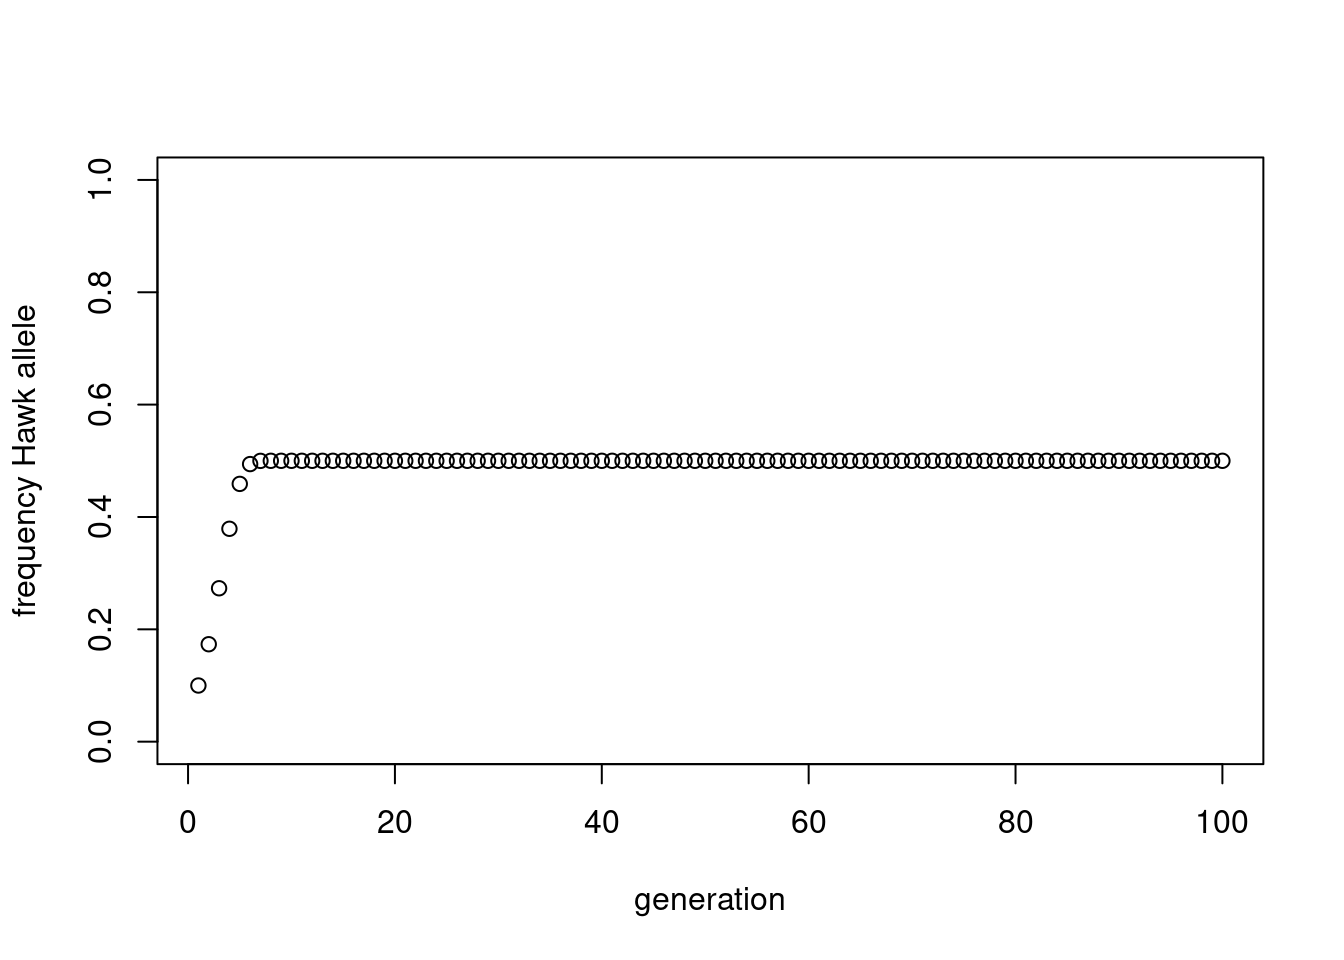
\includegraphics{_main_files/figure-latex/unnamed-chunk-19-1.pdf}

\hypertarget{exercise-5}{%
\section{Exercise}\label{exercise-5}}

From evolutionary game theory, we know that the equilibrium frequency \(\hat{p}\) of hawks (i.e., the frequency at which there is no further change in the frequency of hawks) is \(\hat{p} = v/c\). Do you get the same answer here? What would you conclude about the importance of genetic detail?

\hypertarget{individual-based-simulations-and-drift}{%
\chapter{Individual-based simulations and drift}\label{individual-based-simulations-and-drift}}

Previously, the model of the Hawk-Dove game that we have used was \textbf{deterministic}, where multiple runs for the same values of the parameters \(v\) and \(c\) always result in the same outcome.

In reality, however, evolution does not work like that, as quite a number of biological processes are the result of \textbf{chance}. To give some examples: chance plays a big role in determining whether a mutation occurs or not, whether or not you happen to encounter a hawk rather than a dove, which gamete actually contributes to the next generation or which offspring manages to survive in order to reproduce.

Introducing chance in models of evolution makes these models \textbf{stochastic}, meaning that any two runs of the same model (with the same values of the parameters) does not necessarily result in the same outcome. Stochasticity in evolution introduces a phenomenon called `genetic drift' which we will explore in this practical. Genetic drift can -- particularly in small populations -- dramatically affect the course of evolution!

\hypertarget{before-you-start-this-practical}{%
\section{Before you start this practical}\label{before-you-start-this-practical}}

First, please be reminded to use one of the \href{https://rstudio01.cles.ex.ac.uk}{Rstudio servers} rather than your local installation of R. This is because we will be using some custom-built R packages, which themselves require extensions like \href{https://cran.r-project.org/bin/windows/Rtools/}{Rtools} that can be a bit of a pain to install on some computers. Luckily, this should all have been done for you on the Rstudio server.

Next, when logged in on the Rstudio server, please use R version \texttt{4.1.1.}

And finally, it may be worthwhile to remove variables from our previous session, which we do by typing in the following

\begin{Shaded}
\begin{Highlighting}[]
\CommentTok{\# clean all R variables}
\FunctionTok{rm}\NormalTok{(}\AttributeTok{list=}\FunctionTok{ls}\NormalTok{())}
\end{Highlighting}
\end{Shaded}

\hypertarget{installing-the-driftsim-package}{%
\section{\texorpdfstring{Installing the \texttt{driftSim} package}{Installing the driftSim package}}\label{installing-the-driftsim-package}}

Now, let's get started. In this part of the practical, we will explore a model that includes stochasticity. Such a model is provided in the R package \texttt{driftSim}. To install this package, do the following:

\begin{Shaded}
\begin{Highlighting}[]
\ControlFlowTok{if}\NormalTok{ (}\SpecialCharTok{!}\FunctionTok{require}\NormalTok{(}\StringTok{"devtools"}\NormalTok{)) }\FunctionTok{install.packages}\NormalTok{(}\StringTok{"devtools"}\NormalTok{)}

\FunctionTok{library}\NormalTok{(}\StringTok{"devtools"}\NormalTok{) }
\NormalTok{devtools}\SpecialCharTok{::}\FunctionTok{install\_github}\NormalTok{(}\StringTok{"bramkuijper/driftSim"}\NormalTok{)}
\end{Highlighting}
\end{Shaded}

If you get a message like \texttt{Skipping\ install\ of\ \textquotesingle{}driftSim\textquotesingle{}\ from\ a\ github\ remote,\ the\ SHA1\ (27e9c52c)\ has\ not\ changed\ since\ last\ install.\ Use}force = TRUE\texttt{to\ force\ installation}, R is simply telling you the package has already been installed. Consequently, you can just move on to the next step.

Then we can load the library using:

\begin{Shaded}
\begin{Highlighting}[]
\FunctionTok{library}\NormalTok{(}\StringTok{"driftSim"}\NormalTok{)}
\end{Highlighting}
\end{Shaded}

\hypertarget{individual-based-models}{%
\section{Individual-based models}\label{individual-based-models}}

This package contains what we call an \emph{individual-based simulation}, which is nothing more than a computer program that models individuals and their actions (e.g., surviving, fighting, reproducing). By contrast, in the previous set of exercises, we did not focus on individuals too much, but rather on an \emph{analytical model} which tracked the population-wide frequency \(p_{t}\) of hawks. Indeed, keeping track of a single population-wide frequency \(p_{t}\) is a lot simpler than keeping track of thousands or even millions of individuals. However, such simplicity also comes also at a price, which will be the focus of this chapter.

While the simulation package \texttt{driftSim} runs within R, under the hood it is coded in the low-level programming language \href{https://cplusplus.com/doc/tutorial/}{C++}. This is because large simulations tend to be very slow in R, but run much faster in C++. Below you see a little snippet from this package, reflecting the properties of single individual:

\begin{Shaded}
\begin{Highlighting}[]
\KeywordTok{struct}\NormalTok{ Individual }\OperatorTok{\{}
    \DataTypeTok{bool}\NormalTok{ is\_hawk}\OperatorTok{;} \CommentTok{// TRUE/FALSE individual is hawk or dove}
    \DataTypeTok{double}\NormalTok{ payoff}\OperatorTok{;} \CommentTok{// the value of the payoff}
    \DataTypeTok{double}\NormalTok{ prob\_hawk}\OperatorTok{;} \CommentTok{// the probability that this individual develops as a hawk in early life (only used when strategies are mixed)}
\OperatorTok{\};}
\end{Highlighting}
\end{Shaded}

The program then simulates a \textbf{finite} population of \(N\) of these individuals. You might remember that the analytical model in the previous chapter assumed infinitely many individuals, so while the individual-based model is an absolute loser when it comes to speed, it is already a winner when it comes to increased realism!

\hypertarget{life-cycle-1}{%
\section{Life cycle}\label{life-cycle-1}}

At the start of each generation, each individual interacts with a randomly chosen other individual and either attacks (hawk) or displays (dove). It gets its payoffs based on the same payoff matrix as we used in the deterministic model in the previous chapter. Subsequently, we then produce \(N\) newborn offspring from this population. Parents of each of these offspring are sampled from the previous generation, with individuals who have a larger payoff being more likely to be selected than individuals which have a lower payoff.

\hypertarget{exercise-limiting-assumptions}{%
\section{Exercise: limiting assumptions}\label{exercise-limiting-assumptions}}

Individual-based simulations are often used to relax many of the limiting assumptions present in deterministic models, as writing computer code allows for much more flexibility than when using mathematical formulas. We have already seen how individual-based simulations have relaxed one assumption of the popoulation genetics mode, namely the fact that population sizes can now be finite, rather than infinite.

Can you list three other limiting assumptions from the deterministic population genetics model that you would like to relax? For each assumption, can you think how relaxing the assumption could potentially affect results? (It is often much easier to spell out what is wrong with a model than to spell out how addressing it will change outcomes!)

\hypertarget{running-the-driftsim-package}{%
\section{\texorpdfstring{Running the \texttt{driftSim} package}{Running the driftSim package}}\label{running-the-driftsim-package}}

The \texttt{driftSim} package contains a single function, called \texttt{runSimulation()}. Before running this function, please inspect the documentation by typing \texttt{?runSimulation()} in your R console, after which a help page should show up.

Let us start with a simple example run with a population size of \(N=10\), \(v=1.0\), \(c=2.0\) and a bunch of different parameters. Most are not so important, except that the initial frequency \(p_{t=0}\) of hawks which is set at \(p_{t=0} = 0.25\).

\begin{Shaded}
\begin{Highlighting}[]
\FunctionTok{runSimulation}\NormalTok{(}\AttributeTok{N=}\DecValTok{10}\NormalTok{,}\AttributeTok{v=}\FloatTok{1.0}\NormalTok{,}\AttributeTok{c=}\FloatTok{2.0}\NormalTok{,}\AttributeTok{is\_pure=}\NormalTok{T,}\AttributeTok{mu=}\DecValTok{0}\NormalTok{,}\AttributeTok{max\_time=}\DecValTok{10}\NormalTok{,}\AttributeTok{pHawk\_init=}\FloatTok{0.25}\NormalTok{,}\AttributeTok{output\_nth\_generation=}\DecValTok{1}\NormalTok{,}\AttributeTok{sd\_pHawkMixed=}\DecValTok{0}\NormalTok{)}
\DocumentationTok{\#\#    generation freq\_Hawk mean\_pHawkMixed sd\_pHawkMixed}
\DocumentationTok{\#\# 1           1       0.1               0             0}
\DocumentationTok{\#\# 2           2       0.2               0             0}
\DocumentationTok{\#\# 3           3       0.2               0             0}
\DocumentationTok{\#\# 4           4       0.2               0             0}
\DocumentationTok{\#\# 5           5       0.2               0             0}
\DocumentationTok{\#\# 6           6       0.2               0             0}
\DocumentationTok{\#\# 7           7       0.1               0             0}
\DocumentationTok{\#\# 8           8       0.2               0             0}
\DocumentationTok{\#\# 9           9       0.1               0             0}
\DocumentationTok{\#\# 10         10       0.2               0             0}
\end{Highlighting}
\end{Shaded}

In this way, however, we cannot use the data from the \texttt{runSimulation()} function, as it will simply be printed out to the console, but it is not stored anywhere. To make sure that the resulting data will be contained in a \texttt{data.frame}, we assign the return values from the \texttt{runSimulation()} function to a variable, like this:

\begin{Shaded}
\begin{Highlighting}[]
\NormalTok{my.data }\OtherTok{\textless{}{-}} \FunctionTok{runSimulation}\NormalTok{(}\AttributeTok{N=}\DecValTok{10}\NormalTok{,}\AttributeTok{v=}\FloatTok{1.0}\NormalTok{,}\AttributeTok{c=}\FloatTok{2.0}\NormalTok{,}\AttributeTok{is\_pure=}\NormalTok{T,}\AttributeTok{mu=}\DecValTok{0}\NormalTok{,}\AttributeTok{max\_time=}\DecValTok{10}\NormalTok{,}\AttributeTok{pHawk\_init=}\FloatTok{0.25}\NormalTok{,}\AttributeTok{output\_nth\_generation=}\DecValTok{1}\NormalTok{,}\AttributeTok{sd\_pHawkMixed=}\DecValTok{0}\NormalTok{)}
\end{Highlighting}
\end{Shaded}

The \texttt{my.data} variable points to a \texttt{data.frame} with the following columns:
1. \texttt{generation}: generation time point
2. \texttt{freq\_Hawk}: the frequency of hawks in the population, the variable of interest
3. \texttt{mean\_pHawkMixed}: in case hawks and doves are the result of a mixed strategy, this is the (evolving) probability that any individual will develop as hawk at the start of its life. This is 0 in case \texttt{is\_pure=T}, when we consider pure strategies of hawks and Doves
4. \texttt{sd\_pHawkMixed}: variation among individuals in their ability to develop as hawks (only nonzero when \texttt{is\_pure=F})

\hypertarget{exercise-plotting-the-output-from-the-driftsim-package}{%
\section{\texorpdfstring{Exercise: plotting the output from the \texttt{driftSim} package}{Exercise: plotting the output from the driftSim package}}\label{exercise-plotting-the-output-from-the-driftsim-package}}

Make a plot where plot \texttt{generation} on the \(x\)-axis and \texttt{freq\_Hawk} on the \(y\)-axis. Re-run your simulation at least 10 times. What happens (typically) with the hawk allele?

\hypertarget{exercise-change-the-initial-frequency-of-hawks}{%
\section{Exercise: change the initial frequency of hawks}\label{exercise-change-the-initial-frequency-of-hawks}}

Now, change the initial frequency of hawks by changing the value of \texttt{pHawk\_init} to \texttt{pHawk\_init=0.75}. Run the simulation for a long time, for example \texttt{max\_time=500}. What happens now with the frequency of hawks? What does that tell you about the differences between the analytical model and the current one? Do we still reach the predicted equilibrium frequency of hawks \(\hat{p} = v/c\)?

\hypertarget{exercise-increase-the-population-size}{%
\section{Exercise: increase the population size}\label{exercise-increase-the-population-size}}

Now, try the same with a population size of \(N=500\). What happens now?

\hypertarget{hawk-dove-games-with-relatives}{%
\chapter{Hawk Dove games with relatives}\label{hawk-dove-games-with-relatives}}

So far, we used the Hawk Dove game to study the evolution of fighting behaviour in well-mixed populations. We found that aggression can be limited by costs of fighting \(c\).

In this practical, we take the Hawk Dove game a step further by considering how interactions among relatives affect the evolution of aggression. Indeed, one could argue that a Hawk could be analogous to a defector that exploits cooperative Doves.

In the simple model we used previously, interactions were entirely driven by \emph{random} encounters, so that the probability of encountering one type vs the other was given by the frequencies of Hawks \(p_{t}\) and Doves \(1-p_{t}\) in generation \(t\).

Now we study the case where interactions are not random, but some assortment takes place. Hence, we need to change the model in the same way the prisoner's dilemma model is changed to account for non-random interactions.

While we will use the same payoff matrix as before (see \protect\hyperlink{tab:payoffHD}{the table in chapter 2}), let us now change the interaction probabilities between the individuals. Recall the previous fitness expressions \(W_{H}\) and \(W_{D}\) for Hawks and Doves respectively:
\begin{align}
W_{H} &= w_{0} + p_{t} \frac{v-c}{2} + \left(1 - p_{t} \right) v \label{eq:wH} \\
W_{D} &= w_{0} + p_{t} (0) + \left(1 - p_{t} \right) \frac{v}{2} \label{eq:wD}\\
\end{align}

Below you find the R code that we used to iterate the system of equations.

\begin{Shaded}
\begin{Highlighting}[]
\CommentTok{\# code to iterate a hawk{-}dove game}


\CommentTok{\# parameters coding the payoffs}
\NormalTok{c }\OtherTok{\textless{}{-}} \FloatTok{1.0}
\NormalTok{v }\OtherTok{\textless{}{-}} \DecValTok{0}

\CommentTok{\# baseline fitness}
\NormalTok{w0 }\OtherTok{\textless{}{-}} \DecValTok{10}

\CommentTok{\# maximum time the simulation should run for}
\NormalTok{max\_time }\OtherTok{\textless{}{-}} \DecValTok{1000000}

\CommentTok{\# a vector containing allele frequencies}
\CommentTok{\# for all time steps}
\NormalTok{p }\OtherTok{\textless{}{-}} \FunctionTok{rep}\NormalTok{(}\AttributeTok{x=}\ConstantTok{NA}\NormalTok{, }\AttributeTok{times=}\NormalTok{max\_time)}

\CommentTok{\# set the initial frequency of the hawks}
\CommentTok{\# at time step 1}
\NormalTok{p[[}\DecValTok{1}\NormalTok{]] }\OtherTok{\textless{}{-}} \FloatTok{0.1}

\CommentTok{\# a for loop to iterate the recursion equation}
\CommentTok{\# over multiple timesteps}
\ControlFlowTok{for}\NormalTok{ (time\_idx }\ControlFlowTok{in} \DecValTok{1}\SpecialCharTok{:}\NormalTok{(max\_time}\DecValTok{{-}1}\NormalTok{))}
\NormalTok{\{}
\NormalTok{  wH }\OtherTok{\textless{}{-}}\NormalTok{ w0 }\SpecialCharTok{+}\NormalTok{ p[[time\_idx]] }\SpecialCharTok{*}\NormalTok{ (v}\SpecialCharTok{{-}}\NormalTok{c)}\SpecialCharTok{/}\DecValTok{2} \SpecialCharTok{+}\NormalTok{ (}\DecValTok{1}\SpecialCharTok{{-}}\NormalTok{p[[time\_idx]]) }\SpecialCharTok{*}\NormalTok{ v}
\NormalTok{  wD }\OtherTok{\textless{}{-}}\NormalTok{ w0 }\SpecialCharTok{+}\NormalTok{ p[[time\_idx]] }\SpecialCharTok{*} \DecValTok{0} \SpecialCharTok{+}\NormalTok{ (}\DecValTok{1}\SpecialCharTok{{-}}\NormalTok{p[[time\_idx]]) }\SpecialCharTok{*}\NormalTok{ v}\SpecialCharTok{/}\DecValTok{2}

\NormalTok{  wBar }\OtherTok{\textless{}{-}}\NormalTok{ wH }\SpecialCharTok{*}\NormalTok{ p[[time\_idx]] }\SpecialCharTok{+}\NormalTok{ wD }\SpecialCharTok{*}\NormalTok{ (}\DecValTok{1}\SpecialCharTok{{-}}\NormalTok{p[[time\_idx]])}

  \CommentTok{\# recursion equation}
\NormalTok{  p[[time\_idx }\SpecialCharTok{+} \DecValTok{1}\NormalTok{]] }\OtherTok{\textless{}{-}}\NormalTok{ p[[time\_idx]] }\SpecialCharTok{*}\NormalTok{ wH }\SpecialCharTok{/}\NormalTok{ wBar}
\NormalTok{\}}
\end{Highlighting}
\end{Shaded}

\hypertarget{exercise-running-the-model}{%
\section{Exercise: running the model}\label{exercise-running-the-model}}

Just to get yourself familiar with the model again, try to run it for different values of \(v\) and \(c\) and see what happens.

\hypertarget{interactions-among-relatives}{%
\section{Interactions among relatives}\label{interactions-among-relatives}}

Rather than using the frequencies \(p_{t}\) and \(1-p_{t}\), we will now modify the Hawk Dove game by using \emph{conditional probabilities} reflecting non-random encounter rates, replacing the random encounter rates.

\begin{itemize}
\tightlist
\item
  \[ \Pr(H \mid H)\] probability of encounter between a focal Hawk and non-focal Hawk.
\item
  \[ \Pr(D \mid H)\] probability of encounter between a focal Hawk and a Dove (note again, that \(\Pr(H \mid H) + Pr(D \mid H) = 1\)).
\item
  \[ \Pr(H \mid D)\] probability of encounter between a focal Dove and a Hawk.
\item
  \[ \Pr(D \mid D)\] probability of encounter between a focal Dove and a non-focal Dove (\(\Pr(H \mid D) + \Pr(D \mid D) = 1\)).
\end{itemize}

Incorporating these conditional probabilities into the fitness expressions above yields
\begin{align}
W_{H} &= w_{0} + \Pr(H\mid H) \frac{v-c}{2} +  \Pr (D \mid H ) v \label{eq:wH} \\
W_{D} &= w_{0} + \Pr (H \mid D) (0) + \Pr ( D \mid D )  \frac{v}{2} \label{eq:wD}\\
\end{align}

\hypertarget{hamiltons-rule-in-a-hawk-dove-game}{%
\section{Hamilton's rule in a Hawk Dove game?}\label{hamiltons-rule-in-a-hawk-dove-game}}

If we would follow the example of the Prisoner's dilemma in the lecture slides, would we expect to find something similar to Hamilton's rule when we assess the condition in which more cooperative Doves do better than defecting Hawks, i.e., \(W_{D} > W_{H}\)?

Let us look again at the Prisoner's dilemma: altruists (\(A\)) do better than nonaltruists \(NA\) (originally called `Defect' in the lecture slides but I change notation to avoid confusion with Dove) when \(W_{A} > W_{NA}\), which eventually results in (see lecture slides):
\begin{align}
\left( \Pr(A \mid A ) - \Pr(A \mid NA ) \right ) b &> c \\
\end{align}
where the term \(\Pr(A \mid A ) - \Pr(A \mid NA )\) can be shown to reflect the coefficient of relatedness \(r\).

In case Hamilton's rule would apply to the Hawk Dove game, we would thus expect an expression of the form
\begin{align}
\left(\Pr(D \mid D) - \Pr(D \mid H ) \right ) x &> y \\
\end{align}
where \(x\) and \(y\) would be coefficients that would result from combinations of payoffs in the Hawk Dove game.

Yet, actually working out the same tricks on the Hawk Dove game as was done on the Prisoner's Dilemma in the preceding lecture, we obtain something rather different, namely
\begin{align}
\left [ \Pr (D \mid D) - \Pr ( D \mid H) \right ] v - \Pr (D \mid H) v > \Pr ( H \mid H ) \left (v - c \right )
\end{align}

Clearly, coefficients are not simply \(v\) on the left hand side and \(c\) on the right, but that is obvious as costs are not carried by the cooperators, but rather by pairs of interacting Hawks. But beyond this, there is something more important to note in the expression above, namely that next to the relatedness coefficient \(\Pr(D \mid D) - \Pr(D \mid H )\) there is an additional coefficient on the left-hand side (and the right-hand side is multiplied by \(\Pr(H\mid H)\)).

Hence, rather than anything like \(r x > y\) we now have \(r x + k z > g y\) (i.e., lots more terms)!! And that despite it being a super simple 2 player game! What is going on??

\hypertarget{exercise-the-downfall-of-hamiltons-rule}{%
\section{Exercise: the downfall of Hamilton's rule}\label{exercise-the-downfall-of-hamiltons-rule}}

Can you think of why a simple expression like \(r x > y\) does not apply to the Hawk Dove game? Specifically, compare the payoff matrix for the Prisoner's dilemma (see lecture slides) with the one of the Hawk dove game (see \protect\hyperlink{tab:payoffHD}{the table in chapter 2}). What happens if you move from the top row to the bottom row in the payoff matrix, does the payoff increase / decrease by the same amount in the Hawk Dove game vs the Prisoner's Dilemma? What happens if you move from the left column to the right column? Discuss.

\hypertarget{evolution-of-aggression-when-relatives-interact-in-r}{%
\section{Evolution of aggression when relatives interact in R}\label{evolution-of-aggression-when-relatives-interact-in-r}}

Now that we know we cannot really use Hamilton's rule to predict when Doves will outlive Hawks, we have to resort to our previously used method of iterating a population genetics recursion equation in R to predict how interactions among relatives affects aggression. It turns out, relatedness \(r\) comes into this in another way, namely directly through the conditional probabilities. If we interpret \(r\) as being the chance of interacting with an individual that shares an allele identical by descent, we have

\begin{itemize}
\tightlist
\item
  \[ \Pr(H \mid H) = r \times 1 + (1-r ) p_{t} \] probability of encounter between a focal Hawk and non-focal Hawk.
\item
  \[ \Pr(D \mid H) = r \times 0 + (1-r) (1-p_{t}) \] probability of encounter between a focal Hawk and a Dove (note that \(\Pr(H \mid H) + Pr(D \mid H) = 1\)).
\item
  \[ \Pr(H \mid D) = r \times 0 + (1-r) p_{t} \] probability of encounter between a focal Dove and a Hawk
\item
  \[ \Pr(D \mid D) = r \times 1 + (1- r) (1-p_{t} ) \] probability of encounter between a focal Dove and a non-focal Dove (\(\Pr(H \mid D) + \Pr(D \mid D) = 1\)).
\end{itemize}

\hypertarget{exercise-explaining-these-expressions}{%
\section{Exercise: explaining these expressions?}\label{exercise-explaining-these-expressions}}

Can you try to explain what is going on in the expressions above? Why do allele frequencies \(p_{t}\) still feature here?

\hypertarget{exercise-implementing-it-in-the-numerical-model}{%
\section{Exercise: implementing it in the numerical model}\label{exercise-implementing-it-in-the-numerical-model}}

\begin{enumerate}
\def\labelenumi{\arabic{enumi}.}
\item
  Copy-paste the code of the correct numerical iterations of the hawk dove game above and modify the encounter rates to allow for nonrandom interactions. While \(p_{t}\) is still the allele frequency of the Hawk allele, you have to add \(r\) as a constant parameter, which you can give any value between \(0 \leq r \leq 1\) before you start the iteration. Start with \(r=0.5\), for example, what does this mean about the relatives any individual is most likely to interact?
\item
  Is it reasonable to think as \(r\) as a constant parameter?
\end{enumerate}

\hypertarget{exercise-varying-the-values-of-r}{%
\section{\texorpdfstring{Exercise: varying the values of \(r\)}{Exercise: varying the values of r}}\label{exercise-varying-the-values-of-r}}

Plot your results for different values of \(r\), either in Excel or by using one of the plotting packages in R. Is the relationship between aggression and \(r\) in line with your expectations?

\hypertarget{spatially-explicit-models-of-the-hawk-dove-game}{%
\chapter{Spatially explicit models of the Hawk Dove game}\label{spatially-explicit-models-of-the-hawk-dove-game}}

In the previous set of exercises, we discussed our assumption of \(r\) being constant. While this allows you to assess the role of specific values of \(r\), in reality \(r\) emerges as a result of the ecology of a population, allowing us to focus on the ecological factors that drive the evolution of sociality. Models in which \(r\) is not treated at a constant, but \emph{emerges} are called \emph{demographically consistent}.

One major ecological factor that affects \(r\) is the probability of dispersal: if few individuals disperse, while most just stick around in their natal environment, relatedness among randomly sampled individuals is likely to be much higher than when most individuals disperse and go elsewhere.

\hypertarget{exercise-6}{%
\section{Exercise}\label{exercise-6}}

Can you think of other ecological factors that influence \(r\)?

\hypertarget{investigating-how-dispersal-affects-aggression-adding-space-to-the-hawk-dove-game}{%
\section{Investigating how dispersal affects aggression: adding space to the Hawk Dove game}\label{investigating-how-dispersal-affects-aggression-adding-space-to-the-hawk-dove-game}}

Given the results from the numerical model of the Hawk Dove game among relatives, we would thus predict that reducing the rate of dispersal (which results in an increase in \(r\)) should reduce the evolution of aggression.

To investigate this prediction, we need a model that includes some notion of space, as individuals need to disperse from one patch to another. There lots of different ways to include space in models. Most commonly used are:

\begin{enumerate}
\def\labelenumi{\arabic{enumi}.}
\item
  \textbf{two-patch models}: in which a population distributed across (lo-and-behold) two sites, with migration occurring between them (example: island vs mainland). In this case, at least one of the environments typically contains lots of individuals (the mainland), making it unlikely that relatives encounter each other in a large proportion of the population. If this is the ecological setting, interactions between relatives are likely to be less important anyway.
\item
  \textbf{lattice models}: individuals migrate around on a grid of patches, moving from one patch to an adjacent one per timestep. If this is the ecology, then interactions among relatives are much more likelyt to occur, as even when individuals migrate, they are still close to the natal site and hence likely to interact with other relatives that have dispersed. However, at the same time, this means that what happens in one patches correlates with what happens in another, which makes these models much more tedious to model. Also there are loads of additional assumptions involved (e.g., what do you do at the edge of a lattice? Do you move to the other side (i.e., a torus world) or do you bounce back?
\item
  \textbf{island models}: in this flavour of a spatial model, once individuals migrate, they move to a randomly chosen site in the population. This may well describe taxa such as many insects where individuals move relatively away from their natal patch, while the non-dispersers stay at their natal site. Next to the two-patch case, this is the easiest version of a spatial model, so that is what we will be focusing on here.
\end{enumerate}

\hypertarget{exercise-7}{%
\section{Exercise}\label{exercise-7}}

Discuss the pros and cons of each model - what approach has your preference and why?

The life cycle of the island model is similar to that of the numerical one before: 1. individuals are born; 2. they disperse or not and compete for one of \(N_{bp}\) breeding positions with native and immigrant juveniles; 3. they interact with a randomly chosen patch mate and obtain a payoff; 4. the number of offspring that are produced are then proportional to the payoff they have received.

\hypertarget{a-spatial-model-of-the-hawk-dove-game}{%
\section{A spatial model of the hawk dove game}\label{a-spatial-model-of-the-hawk-dove-game}}

In \texttt{R} (make sure you use version 4.1.1), we now proceed to install the package \texttt{hdIslandModel} which is an individual based simulation of an island model with Hawks and Doves, allowing us to vary the rate of dispersal.

\begin{Shaded}
\begin{Highlighting}[]
\ControlFlowTok{if}\NormalTok{ (}\SpecialCharTok{!}\FunctionTok{require}\NormalTok{(}\StringTok{"devtools"}\NormalTok{)) }\FunctionTok{install.packages}\NormalTok{(}\StringTok{"devtools"}\NormalTok{)}

\FunctionTok{library}\NormalTok{(}\StringTok{"devtools"}\NormalTok{)}
\NormalTok{devtools}\SpecialCharTok{::}\FunctionTok{install\_github}\NormalTok{(}\StringTok{"bramkuijper/hdIslandModel"}\NormalTok{)}
\end{Highlighting}
\end{Shaded}

Then we can load the library using:

\begin{Shaded}
\begin{Highlighting}[]
\FunctionTok{library}\NormalTok{(}\StringTok{"hdIslandModel"}\NormalTok{)}
\end{Highlighting}
\end{Shaded}

The model contained in the package can be called by the command \texttt{runHDSpace()} which spits out a \texttt{data.frame} containing a bunch of statistics resulting from the simulation that we can save in a variable, say \texttt{sim.standard}:

\begin{Shaded}
\begin{Highlighting}[]
\NormalTok{sim.standard }\OtherTok{\textless{}{-}} \FunctionTok{runHDSpace}\NormalTok{() }
\end{Highlighting}
\end{Shaded}

\hypertarget{exercise-8}{%
\section{Exercise}\label{exercise-8}}

\begin{enumerate}
\def\labelenumi{\arabic{enumi}.}
\item
  Take a look at the documentation of the function \texttt{runHDSpace()} by typing \texttt{?runHDSpace()}.
\item
  Let's run the island model for a payoff in which we would expect an evolutionarily stable strategy (ESS) to occur at \(\hat{p}=0.5\) (frequency Hawks is 50\%) when interactions among relatives are absent. This happens happens when \(\hat{p} = v/c = 1/2\). To run the model, focus on a pure strategy (do you remember what this means?) with a small mutation rate of \(mu=0.01\) and \(N=10\) breeders patch. Set the dispersal rate to something low, like \(d=0.1\), which typically results in quite high relatedness coefficients of \(r\approx 0.3-0.4\) among randomly sampled patch mates. The other parameters can be left at their default values.
\item
  In case dispersal indeed increases \(r\), what would we expect to see happen with the proportion of Hawks over time, should it be smaller or larger than 0.5? What is the proportion of Hawks at the end of the simulation? (Run multiple runs, as drift may cause outcomes to vary).
\item
  What happens if you set the dispersal rate to \(d=0.8\)? Does this make a difference?
\end{enumerate}

\hypertarget{exercise-9}{%
\section{Exercise}\label{exercise-9}}

What can we conclude about the relationship between dispersal and social behaviour from the above? Why does this happen, you think?

\hypertarget{exercise-10}{%
\section{Exercise}\label{exercise-10}}

Perhaps something different happens if we allow dispersal to evolve? Run your simulation for \(max_time = 20000\) and see what happens with the dispersal rate. Does dispersal evolve in a predictable way?

\hypertarget{exercise-11}{%
\section{Exercise}\label{exercise-11}}

Now incorporate the modulated

\end{document}
